% Options for packages loaded elsewhere
\PassOptionsToPackage{unicode}{hyperref}
\PassOptionsToPackage{hyphens}{url}
\PassOptionsToPackage{dvipsnames,svgnames,x11names}{xcolor}
%
\documentclass[
  10pt,
]{article}
\usepackage{amsmath,amssymb}
\usepackage{iftex}
\ifPDFTeX
  \usepackage[T1]{fontenc}
  \usepackage[utf8]{inputenc}
  \usepackage{textcomp} % provide euro and other symbols
\else % if luatex or xetex
  \usepackage{unicode-math} % this also loads fontspec
  \defaultfontfeatures{Scale=MatchLowercase}
  \defaultfontfeatures[\rmfamily]{Ligatures=TeX,Scale=1}
\fi
\usepackage{lmodern}
\ifPDFTeX\else
  % xetex/luatex font selection
\fi
% Use upquote if available, for straight quotes in verbatim environments
\IfFileExists{upquote.sty}{\usepackage{upquote}}{}
\IfFileExists{microtype.sty}{% use microtype if available
  \usepackage[]{microtype}
  \UseMicrotypeSet[protrusion]{basicmath} % disable protrusion for tt fonts
}{}
\makeatletter
\@ifundefined{KOMAClassName}{% if non-KOMA class
  \IfFileExists{parskip.sty}{%
    \usepackage{parskip}
  }{% else
    \setlength{\parindent}{0pt}
    \setlength{\parskip}{6pt plus 2pt minus 1pt}}
}{% if KOMA class
  \KOMAoptions{parskip=half}}
\makeatother
\usepackage{xcolor}
\usepackage[margin=0.78in]{geometry}
\usepackage{longtable,booktabs,array}
\usepackage{calc} % for calculating minipage widths
% Correct order of tables after \paragraph or \subparagraph
\usepackage{etoolbox}
\makeatletter
\patchcmd\longtable{\par}{\if@noskipsec\mbox{}\fi\par}{}{}
\makeatother
% Allow footnotes in longtable head/foot
\IfFileExists{footnotehyper.sty}{\usepackage{footnotehyper}}{\usepackage{footnote}}
\makesavenoteenv{longtable}
\usepackage{graphicx}
\makeatletter
\def\maxwidth{\ifdim\Gin@nat@width>\linewidth\linewidth\else\Gin@nat@width\fi}
\def\maxheight{\ifdim\Gin@nat@height>\textheight\textheight\else\Gin@nat@height\fi}
\makeatother
% Scale images if necessary, so that they will not overflow the page
% margins by default, and it is still possible to overwrite the defaults
% using explicit options in \includegraphics[width, height, ...]{}
\setkeys{Gin}{width=\maxwidth,height=\maxheight,keepaspectratio}
% Set default figure placement to htbp
\makeatletter
\def\fps@figure{htbp}
\makeatother
\setlength{\emergencystretch}{3em} % prevent overfull lines
\providecommand{\tightlist}{%
  \setlength{\itemsep}{0pt}\setlength{\parskip}{0pt}}
\setcounter{secnumdepth}{-\maxdimen} % remove section numbering
\usepackage{amsmath,amssymb,mathtools,bm}
\usepackage{booktabs,longtable,array}
\usepackage{graphicx,float}
\graphicspath{{/mnt/data/}}
\usepackage{xcolor}
\usepackage{hyperref}
\usepackage{microtype}
\definecolor{deepblue}{HTML}{1F4E79}
\hypersetup{colorlinks=true,linkcolor=deepblue,urlcolor=deepblue,citecolor=deepblue}
\setlength{\parindent}{0pt}
\setlength{\parskip}{5pt plus 1pt minus 1pt}
\renewcommand{\arraystretch}{1.15}
\ifLuaTeX
  \usepackage{selnolig}  % disable illegal ligatures
\fi
\usepackage{bookmark}
\IfFileExists{xurl.sty}{\usepackage{xurl}}{} % add URL line breaks if available
\urlstyle{same}
\hypersetup{
  pdftitle={Exact Transient Matching and Nonlinear Reheating Cascade},
  pdfauthor={Technical Research Note v1.2},
  colorlinks=true,
  linkcolor={blue},
  filecolor={Maroon},
  citecolor={Blue},
  urlcolor={blue},
  pdfcreator={LaTeX via pandoc}}

\title{Exact Transient Matching and Nonlinear Reheating Cascade}
\usepackage{etoolbox}
\makeatletter
\providecommand{\subtitle}[1]{% add subtitle to \maketitle
  \apptocmd{\@title}{\par {\large #1 \par}}{}{}
}
\makeatother
\subtitle{Factorised three-loop matching, spurion-graded operator
mixing, and the \(\phi\to N_0\bar N_0\to R_0\nu_0\) two-sector plasma
cascade}
\author{Technical Research Note v1.2}
\date{18 August 2026}

\begin{document}
\maketitle

{
\hypersetup{linkcolor=}
\setcounter{tocdepth}{3}
\tableofcontents
}
\section{Executive verdict}\label{executive-verdict}

The v1.2 calculation gives a \textbf{pass for the factorised matching
problem}, a \textbf{qualified pass for the transient operator
renormalisation problem}, and a \textbf{pass for the nonlinear radial
momentum-lattice benchmark}. It does not yet constitute a full
non-Abelian, two-time, \(3+1\)-dimensional Kadanoff-Baym simulation.

The first selector-threshold graph identified in v1.1 is three-loop and
one-particle irreducible, but it is two-particle reducible. That fact is
decisive: its zero-external-momentum matching coefficient does not
require an unknown generic three-loop master integral. It factorises
into:

\begin{enumerate}
\def\labelenumi{\arabic{enumi}.}
\tightlist
\item
  a finite one-loop selector-reheaton-Higgs kernel; and
\item
  a mixed mass derivative of the known two-loop fermion-fermion-scalar
  effective-potential function.
\end{enumerate}

In the explicitly normalised scalar proxy used here,

\[
\boxed{
\mathcal I_3(\bar\mu)
=
2m_R^2K_{RRH}(m_R^2,m_h^2)
D_{FFS}(M^2,m_h^2;\bar\mu)
}
\]

and at the natural hard matching scale \(\bar\mu=M\),

\[
\boxed{
\mathcal I_3(M)=6.57973508149
\simeq
\frac{2\pi^2}{3}.
}
\]

The resulting transient selector-phase potential has benchmark amplitude

\[
\boxed{
|\Delta V_{Qa}^{(3)}|
=2.1723\times10^3\ {\rm GeV}^4,
}
\]

which is only

\[
\boxed{
1.546\times10^{-12}
}
\]

of the intended finite-density reheating force. The first mixed vacuum
correction is therefore negligible in the benchmark.

The anomalous-dimension audit also corrects one overstatement in v1.1.
Exact \(Z_6\) symmetry \textbf{does not by itself make the complete
invariant transient-operator basis block diagonal to all orders}. The
correct statement is:

\[
\boxed{
\gamma_{(A,p)(B,q)}
=
\sum_{r,s\ge0}
\delta_{p-q,r-s}\,
\epsilon^{r+s}
\Gamma_{AB}^{(r,s)},
}
\]

with replica Fourier charge conserved modulo six. It is block diagonal
at order \(\epsilon^0\); changing harmonic \(q\to p\) requires the
corresponding number of shift-breaking spurion insertions. For the
cosmological benchmark \(\epsilon=2.7\times10^{-13}\), the first
cross-harmonic entries are consequently negligible, but the finite
gauge/Yukawa tensors \(\Gamma_{AB}^{(r,s)}\) remain model-dependent and
have not all been computed.

The nonlinear momentum-lattice evolution resolves the chain

\[
\phi
\longrightarrow
N_0\bar N_0
\longrightarrow
R_0\nu_0
\longrightarrow
H_0,H_5
\longrightarrow
D_k,q_k,g_k
\]

with expansion, Pauli blocking, time-dilated two-body decays, exact
isotropic decay kinematics on a radial momentum grid, and an
energy-conserving quantum-BGK thermalisation closure.

It finds:

\[
\boxed{
\frac{\rho_N}{\rho_{\rm tot}}\bigg|_{\rm preheat}
=9.2845\times10^{-8},
\qquad
\max f_N=0.999929,
}
\]

and an unselected-replica production bound of approximately

\[
\log_{10}P_{N_h}<-8562.6.
\]

The cascade exposes one mandatory correction to v0.9-v1.1. The decay
\(N_0\to R_0\nu_0\) deposits the energetic \(\nu_0\) daughter into
sector 0 before \(R_0\) decays. The old choice \(\tan\theta=1/16\),
equivalent to \(B_5=1/257\), therefore does \textbf{not} produce
\(T_5/T_0=1/4\). The full lattice gives the redshift-corrected branch

\[
\boxed{
B_5=0.00527437084,
\qquad
\tan\theta=0.0728196,
}
\]

and

\[
\boxed{
\frac{T_5}{T_0}=0.250000001.
}
\]

The maximum two-body kinematic energy residual is \(5.59\times10^{-16}\)
and the maximum collision-step energy residual is
\(1.73\times10^{-16}\).

The strongest defensible conclusion is therefore:

\[
\boxed{
\begin{gathered}
\text{the first mixed selector-threshold correction is calculable and tiny,}\\
\text{the state-selected fermionic cascade preserves the desired replica hierarchy,}\\
\text{and no radiative or nonlinear failure appears at the resolved level.}
\end{gathered}
}
\]

The remaining frontier is not an unidentified \(\mathcal I_3\). It is
the full RG-improved operator basis and the replacement of the BGK
plasma closure by genuine non-Abelian collision or 2PI/Kadanoff-Baym
kernels.

\section{1. Model and matching
normalisation}\label{model-and-matching-normalisation}

\subsection{1.1 Scalar proxy for the mixed
topology}\label{scalar-proxy-for-the-mixed-topology}

The calculation isolates the selector-threshold topology with the
interaction normalisation

\[
\begin{aligned}
\mathcal L_{\rm proxy}\supset{}&
-\frac12
\left(m_R^2+\lambda_{QR}\mathcal Q\right)R^2
-\frac{\mu_H}{2}Rh^2
-y_Dh\bar qD
-M(a)\bar DD,
\end{aligned}
\]

where

\[
x\equiv\frac a{f_a},
\qquad
M(a)=M\left[1-\epsilon\cos x\right],
\]

so that, to first order in \(\epsilon\),

\[
\delta M^2(a)=-2\epsilon M^2\cos x.
\]

The selector Fourier composite carrying the compensating \(Z_6\) charge
is denoted schematically by \(\mathcal Q\). On the one-hot branch used
in cosmology, \(\mathcal Q\to v_Q^2\) up to its phase convention.

This proxy deliberately does not claim every Standard Model
Higgs-doublet, colour, gauge, and chiral multiplicity. It fixes the
scalar normalisation in which the factorisation and benchmark
coefficient are exact. A complete model matching can be obtained by
restoring the appropriate group-theory and field-multiplicity factors.

\subsection{1.2 Why the graph
factorises}\label{why-the-graph-factorises}

The microscopic graph contains:

\begin{itemize}
\tightlist
\item
  one selector insertion in an \(R\) propagator;
\item
  two \(Rhh\) vertices;
\item
  two Yukawa vertices joining \(h\), \(q\), and \(D\);
\item
  one phase-dependent insertion in the heavy \(D\) mass.
\end{itemize}

Its graph count is

\[
I=8,
\qquad
V=6,
\qquad
L=I-V+1=3.
\]

It is 1PI but two-particle reducible. At zero external momentum, cutting
the two Higgs lines separates the selector-reheaton loop from the
two-loop \(FFS\) vacuum skeleton. The matching therefore takes the form

\[
\Delta V_{Qa}^{(3)}
=
\frac{N_cy_D^2}{(16\pi^2)^2}
\frac{\partial^2f_{FFS}}{\partial M^2\partial m_h^2}
\delta M^2(a)\,
\delta m_h^2(\mathcal Q),
\]

where the selector-generated Higgs mass insertion is

\[
\delta m_h^2(\mathcal Q)
=
\frac{\lambda_{QR}\mu_H^2}{16\pi^2}
K_{RRH}(m_R^2,m_h^2)\mathcal Q.
\]

Generic three-loop vacuum diagrams with arbitrary masses require
integration-by-parts reduction to a master basis and numerical tools
such as 3VIL. The topology here is simpler because its 2PR structure
exposes the factorisation before such a reduction is required.

\section{2. Exact factorised three-loop
coefficient}\label{exact-factorised-three-loop-coefficient}

\subsection{2.1 One-loop selector
kernel}\label{one-loop-selector-kernel}

The finite Euclidean kernel, with the overall \(1/(16\pi^2)\) removed,
is

\[
\boxed{
K_{RRH}(A,B)
=
\frac{A-B-B\ln(A/B)}{(A-B)^2}.
}
\]

It corresponds to

\[
\int\frac{d^4p}{(2\pi)^4}
\frac{1}{(p^2+A)^2(p^2+B)}.
\]

The equal-mass limit is smooth:

\[
K_{RRH}(A,A)=\frac{1}{2A}.
\]

For the benchmark hierarchy \(m_R\gg m_h\),

\[
m_R^2K_{RRH}(m_R^2,m_h^2)
=0.999999999999517.
\]

\subsection{2.2 Mixed derivative of the two-loop FFS
function}\label{mixed-derivative-of-the-two-loop-ffs-function}

In Martin's two-loop effective-potential notation,

\[
f_{FFS}(x,0,z)
=-J(x,z)+(x-z)I(0,x,z).
\]

Taking the exact mixed derivative gives

\[
\boxed{
\begin{aligned}
D_{FFS}(x,z;\bar\mu)
\equiv{}&
\frac{\partial^2f_{FFS}(x,0,z)}{\partial x\partial z}
\\[1mm]
={}&
2\ln\frac{x}{z}
\ln\frac{x-z}{\bar\mu^2}
-
\ln^2\frac{x}{\bar\mu^2}
-
2\operatorname{Li}_2\left(\frac zx\right)
+
\frac{\pi^2}{3}.
\end{aligned}
}
\]

The symbolic residual between this expression and the derivative of the
full \(I(0,x,z)\) representation is exactly zero.

At the hard scale \(\bar\mu=M\) and for \(z/x\to0\),

\[
D_{FFS}\longrightarrow\frac{\pi^2}{3}.
\]

The benchmark gives

\[
D_{FFS}(M^2,m_h^2;M)=3.28986754075,
\]

with a 70-digit independent derivative check agreeing to relative error

\[
4.05\times10^{-16}.
\]

\subsection{2.3 Exact matching function}\label{exact-matching-function}

Combining the two factors defines

\[
\boxed{
\mathcal I_3(\bar\mu)
=
2m_R^2
K_{RRH}(m_R^2,m_h^2)
D_{FFS}(M^2,m_h^2;\bar\mu).
}
\]

The three-loop Wilson coefficient is

\[
\boxed{
C_3^{\overline{\rm MS}}(\bar\mu)
=
\frac{N_c\lambda_{QR}y_D^2}{(16\pi^2)^3}
\frac{\mu_H^2M^2}{m_R^2}
\mathcal I_3(\bar\mu).
}
\]

The transient operator is then

\[
\Delta V_{Qa}^{(3)}
=
\epsilon C_3^{\overline{\rm MS}}
\operatorname{Re}\left[e^{ix}\mathcal Q_{-1}\right]
+O(\epsilon^2).
\]

For

\[
\begin{gathered}
N_c=3,
\quad
\lambda_{QR}=0.50,
\quad
y_D=0.30,
\quad
\mu_H=1.8848\times10^4\ {\rm GeV},\\
M=1.002\times10^6\ {\rm GeV},
\quad
m_R=10^9\ {\rm GeV},
\quad
m_h=125.25\ {\rm GeV},
\end{gathered}
\]

one obtains

\[
\mathcal I_3(M)=6.57973508149,
\]

\[
C_3(M)=8.04542\times10^{-5}\ {\rm GeV}^2.
\]

With

\[
\epsilon=2.70\times10^{-13},
\qquad
v_Q=10^{10}\ {\rm GeV},
\]

this gives

\[
|\Delta V_{Qa}^{(3)}|
=2.1723\times10^3\ {\rm GeV}^4.
\]

The intended state-dependent thermal focusing potential is approximately

\[
V_{\rm thermal}=1.4053\times10^{15}\ {\rm GeV}^4,
\]

hence

\[
\frac{|\Delta V_{Qa}^{(3)}|}{V_{\rm thermal}}
=1.5458\times10^{-12}.
\]

\begin{figure}
\centering
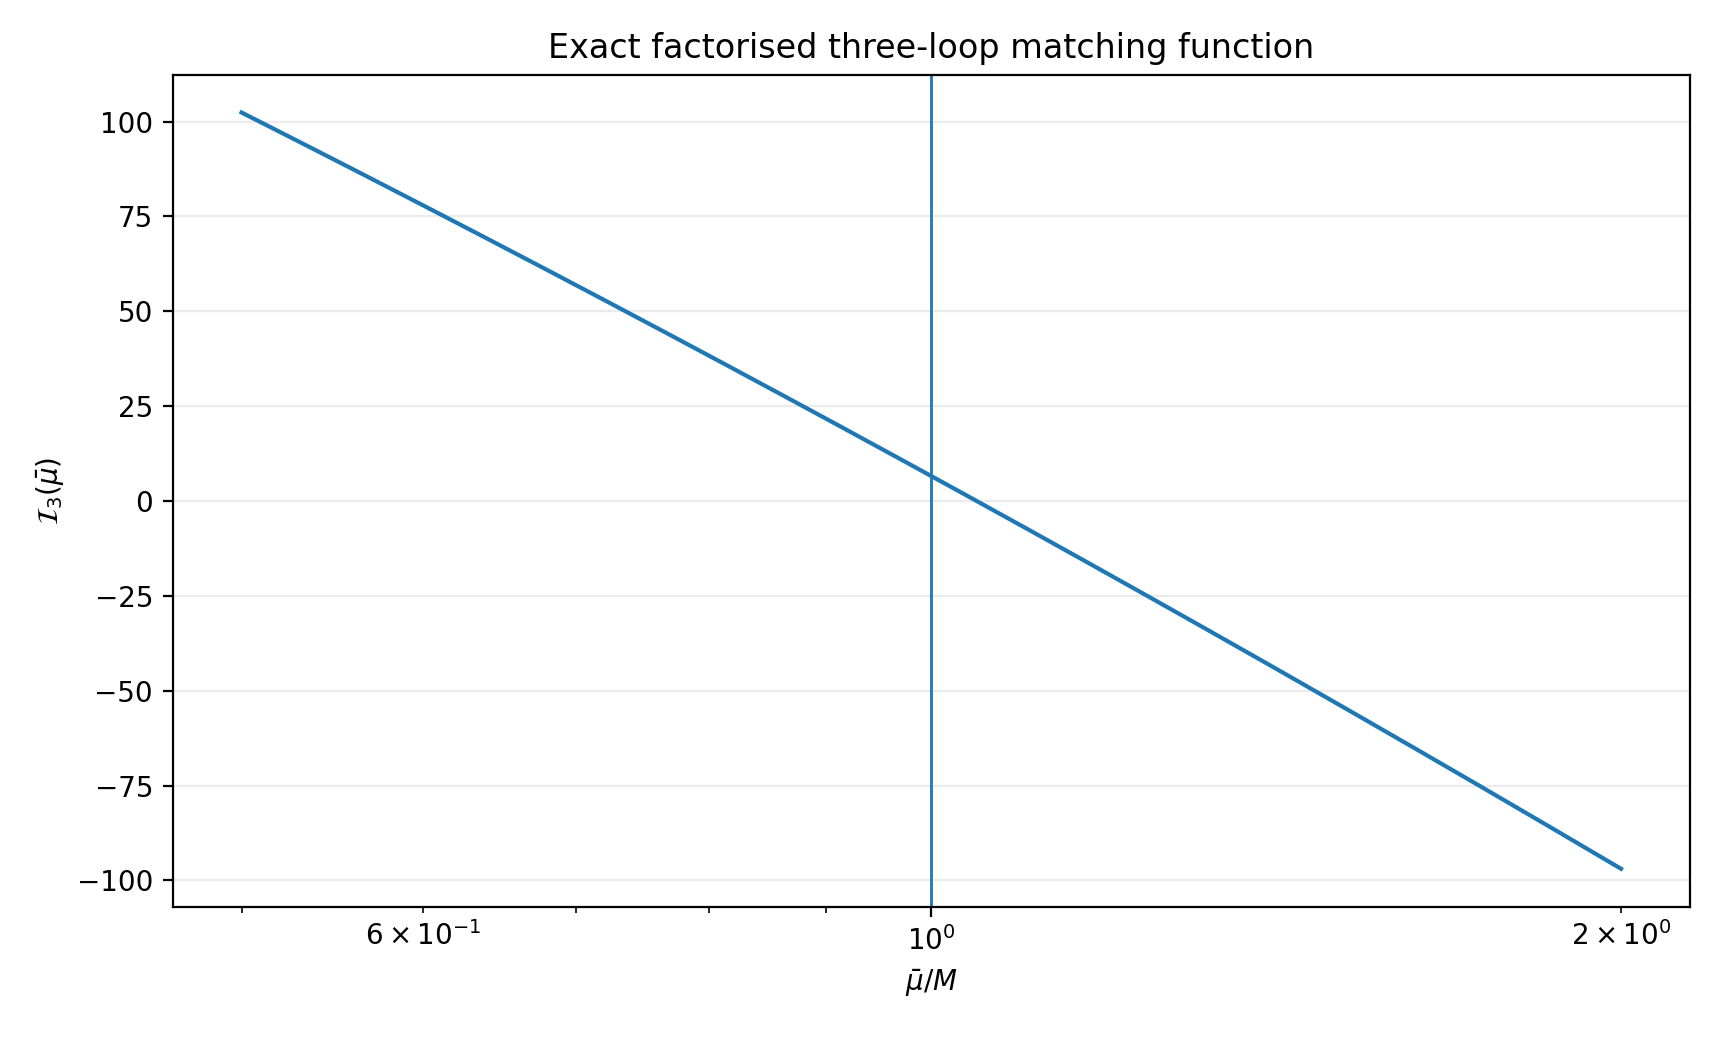
\includegraphics[width=0.86\textwidth,height=\textheight]{exact_three_loop_matching_v1_2.png}
\caption{The exact factorised matching function. Its large residual
scale dependence away from \(\bar\mu=M\) is matching-scale dependence
that must be cancelled by RG evolution, not a physical error band.}
\end{figure}

\subsection{2.4 Scale dependence and what remains to be
matched}\label{scale-dependence-and-what-remains-to-be-matched}

The fixed-order values are

\[
\mathcal I_3(M/2)=102.4073,
\qquad
\mathcal I_3(M)=6.57974,
\qquad
\mathcal I_3(2M)=-96.9351.
\]

This large scale variation reflects the hierarchy \(m_R\gg M\gg m_h\)
and the absence of RG improvement in the displayed coefficient. It must
not be interpreted as a physical uncertainty band. A complete
calculation should:

\begin{enumerate}
\def\labelenumi{\arabic{enumi}.}
\tightlist
\item
  match at the heavy scales;
\item
  evolve the transient operator basis between \(m_R\), \(M\), and
  \(m_h\);
\item
  include finite gauge, chiral, and Higgs-doublet multiplicities; and
\item
  verify cancellation of \(\bar\mu\) dependence in the physical focusing
  force.
\end{enumerate}

The exact result delivered here is the hard zero-momentum matching
function in the scalar proxy.

\section{3. Transient anomalous
dimensions}\label{transient-anomalous-dimensions}

\subsection{3.1 Combined symmetry and operator
basis}\label{combined-symmetry-and-operator-basis}

Let the exact generator act as

\[
z:
\quad
x\to x+\frac{2\pi}{6},
\qquad
k\to k+1.
\]

For a replica Fourier composite

\[
\mathcal X_{A,p}
=
\sum_{k=0}^{5}
X_{A,k}\,e^{-2\pi ipk/6},
\]

one has

\[
\mathcal X_{A,p}\to e^{2\pi ip/6}\mathcal X_{A,p}.
\]

A transient invariant can therefore be written as

\[
\mathcal O_{A,p}
=
e^{ipx}\mathcal X_{A,-p}.
\]

Every \(\mathcal O_{A,p}\) is invariant under the exact combined
\(Z_6\). Consequently, \(Z_6\) invariance alone does not distinguish
different \(p\) values inside the invariant basis.

The additional grading comes from the restored continuous shift symmetry
in the limit \(\epsilon\to0\). Let a positive and negative
shift-breaking insertion carry charges \(+1\) and \(-1\). Renormalising
harmonic \(q\) into harmonic \(p\) requires integers \(r,s\ge0\)
satisfying

\[
r-s=p-q.
\]

Therefore the exact spurion expansion is

\[
\boxed{
\gamma_{(A,p)(B,q)}
=
\sum_{r,s\ge0}
\delta_{p-q,r-s}
\epsilon^{r+s}
\Gamma_{AB}^{(r,s)},
}
\]

with the corresponding replica charge conserved modulo six.

At leading order,

\[
\boxed{
\gamma_{(A,p)(B,q)}
=
\delta_{pq}
\left[
\Gamma_{\rm quad}^{T}
+p\gamma_\epsilon\mathbf1
\right]
+O(\epsilon).
}
\]

The earlier claim of exact all-orders block diagonality was therefore
too strong. The corrected statement is stronger physically and weaker
algebraically:

\[
\boxed{
q\to p\text{ mixing begins at the minimum permitted power of }\epsilon.
}
\]

For sectors folded modulo six, the minimum power is

\[
d_6(p-q)=\min\left(|p-q|,6-|p-q|\right).
\]

Integer harmonic grading must still be retained: the neutral vacuum
harmonic \(p=6\) begins at \(\epsilon^6\), even though
\(6\equiv0\pmod6\).

\subsection{3.2 Explicit one-loop scalar
block}\label{explicit-one-loop-scalar-block}

For real scalar variables with convention

\[
V_4
=
\sum_i\frac{\lambda_i}{4!}X_i^4
+
\sum_{i<j}\frac{\lambda_{ij}}4X_i^2X_j^2,
\]

the one-loop bilinear block before gauge and Yukawa additions is

\[
\Gamma_{\rm quad}^{(0,0)}
=
\frac1{16\pi^2}
\begin{pmatrix}
\lambda_Q&\lambda_{QR}&\lambda_{QH}\\
\lambda_{QR}&\lambda_R&\lambda_{RH}\\
\lambda_{QH}&\lambda_{RH}&\lambda_H
\end{pmatrix}.
\]

For the diagnostic couplings

\[
(\lambda_Q,\lambda_R,\lambda_H)
=(0.10,0.20,0.13),
\]

\[
(\lambda_{QR},\lambda_{QH},\lambda_{RH})
=(0.50,0,0.05),
\]

this is

\[
\Gamma_{\rm quad}^{(0,0)}
=
\begin{pmatrix}
6.3326\times10^{-4}&3.1663\times10^{-3}&0\\
3.1663\times10^{-3}&1.2665\times10^{-3}&3.1663\times10^{-4}\\
0&3.1663\times10^{-4}&8.2323\times10^{-4}
\end{pmatrix}.
\]

At \(\epsilon=2.7\times10^{-13}\), a nearest-harmonic entry with a
coefficient comparable to the largest scalar-block entry is at most of
order

\[
8.55\times10^{-16}.
\]

\begin{figure}
\centering
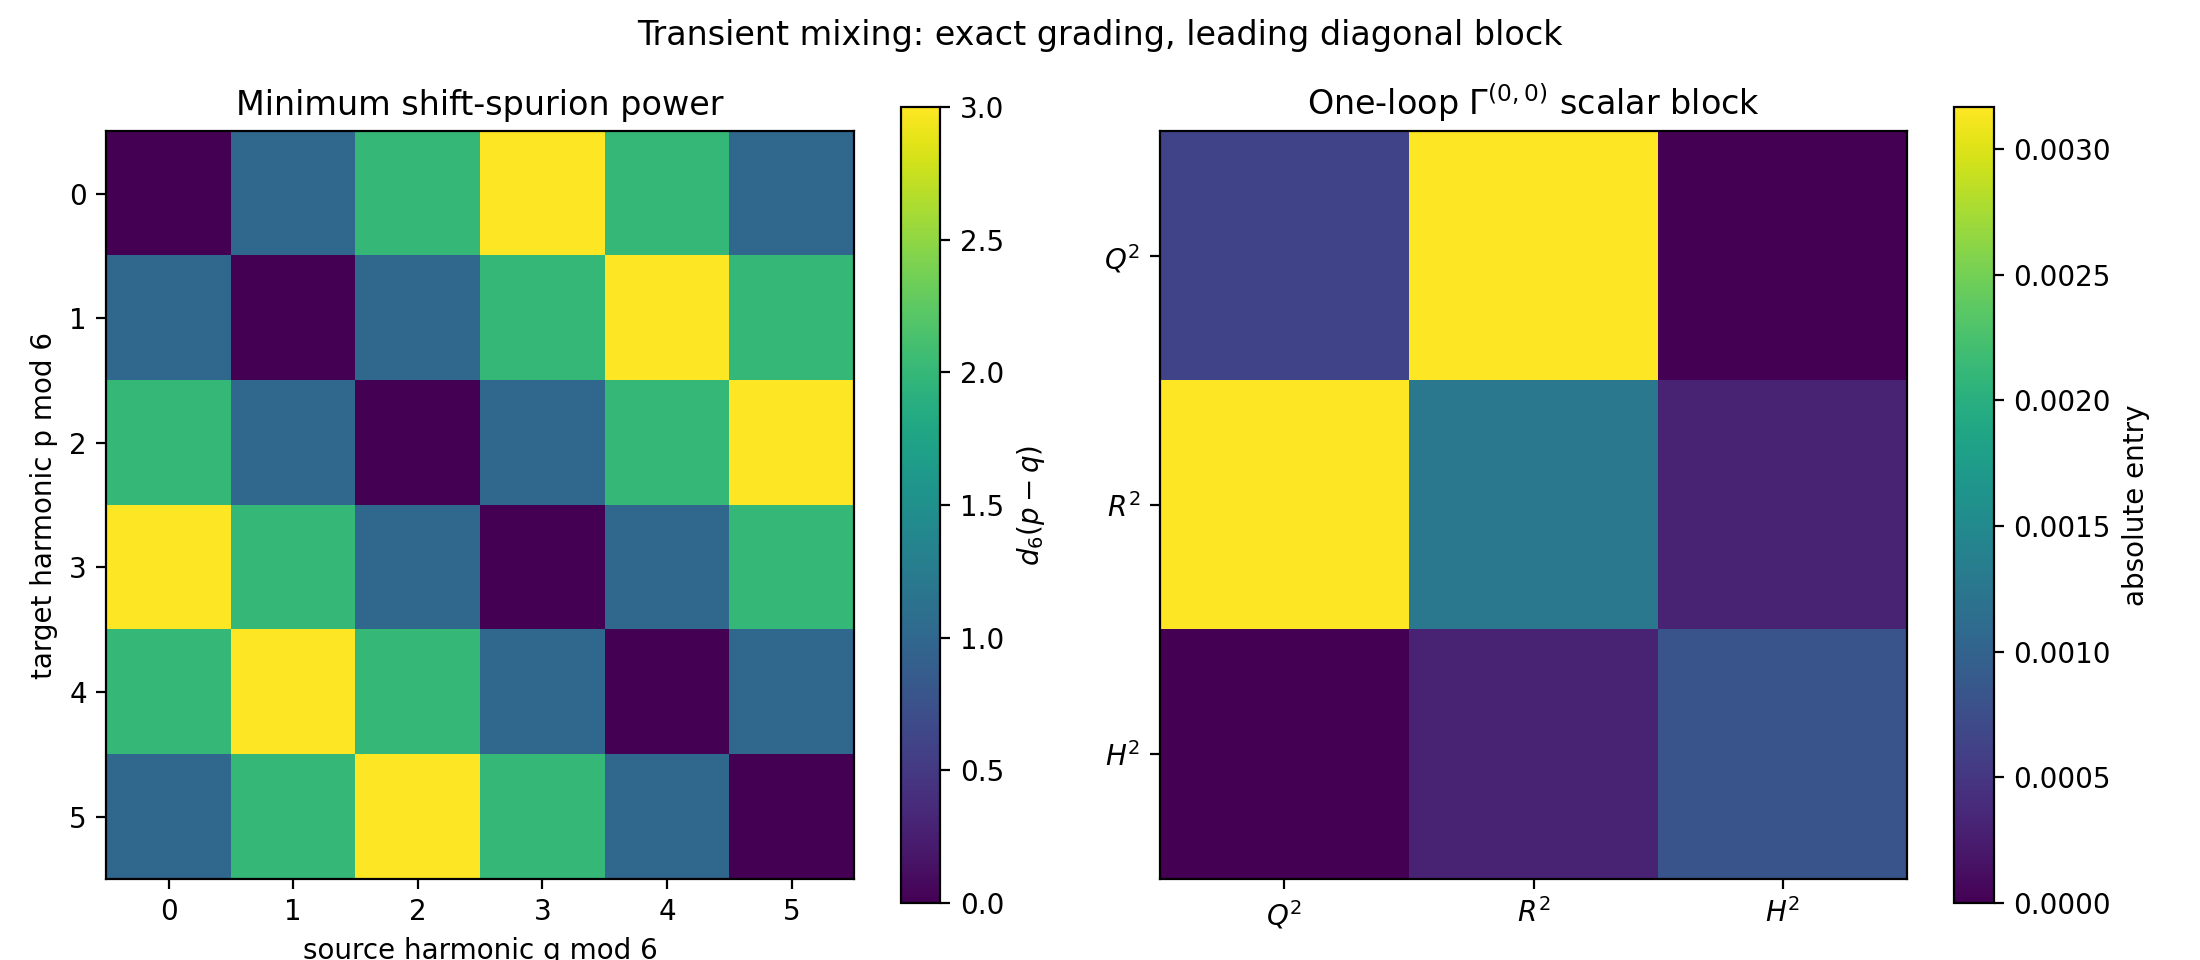
\includegraphics[width=0.98\textwidth,height=\textheight]{transient_gamma_blocks_v1_2.png}
\caption{The exact spurion-power grading and the explicitly calculated
leading scalar bilinear block.}
\end{figure}

\subsection{3.3 Local operators versus state
harmonics}\label{local-operators-versus-state-harmonics}

The local Wilson coefficients obey

\[
\mu\frac{dC_{A,p}}{d\mu}
=
\sum_{B,q}
\gamma_{(A,p)(B,q)}C_{B,q}.
\]

The occupation harmonics

\[
\mathcal N_p(t,\mathbf k)
=
\sum_k n_k(t,\mathbf k)e^{-2\pi ipk/6}
\]

are not governed by this local anomalous-dimension matrix. Their
evolution is determined by Kadanoff-Baym or collision kernels. Confusing
these two kinds of evolution would conflate vacuum renormalisation with
finite-density transport.

The full finite \(\Gamma_{AB}^{(r,s)}\) tensors involving gauge, Yukawa,
fermion bilinear, and gluonic operators remain an open calculation. The
symmetry-imposed power structure is exact; the complete coefficients are
not yet known.

\section{4. Fermionic preheating
stage}\label{fermionic-preheating-stage}

\subsection{4.1 Successive zero-crossing
map}\label{successive-zero-crossing-map}

The selected fermionic parent has

\[
\mathcal L\supset-y_\phi\phi\bar N_0N_0,
\]

with benchmark

\[
m_\phi=10^{10}\ {\rm GeV},
\quad
\Phi_{\rm end}=5.96\times10^{16}\ {\rm GeV},
\quad
m_{N_0}=3\times10^9\ {\rm GeV},
\]

\[
y_\phi=7.006\times10^{-4}.
\]

At each inflaton zero crossing, the Landau-Zener probability is
represented by

\[
P_p
=
\exp\left[
-\pi\frac{p^2+m_N^2}{y_\phi m_\phi\Phi}
\right].
\]

The stochastic Pauli-limited update is

\[
\boxed{
f_N^{j+1}(p)
=
P_p+
\left(1-2P_p\right)f_N^j(p),
}
\]

followed by expansion and energy backreaction on the inflaton
condensate. This preserves

\[
0\le f_N\le1.
\]

Fermionic preheating is nonperturbative but differs sharply from bosonic
resonance because Pauli blocking prevents unbounded occupation growth.

\subsection{4.2 Numerical result}\label{numerical-result}

The calculation uses 320 zero crossings and a 280-bin logarithmic
comoving momentum grid. It finds

\[
\max f_N=0.999929,
\]

but only

\[
\boxed{
\frac{\rho_N}{\rho_\phi+\rho_N}
=9.2845\times10^{-8}
}
\]

at the end of the preheating stage. The early nonperturbative component
is therefore dynamically negligible compared with the subsequent
perturbative decay.

The hidden parent mass is

\[
m_{N_h}=5\times10^{13}\ {\rm GeV}.
\]

Its smallest Landau-Zener exponent during the evolution is

\[
\pi\frac{m_{N_h}^2}{y_\phi m_\phi\Phi}
=1.9716\times10^4,
\]

implying

\[
\boxed{
\log_{10}P_{N_h}<-8562.6.
}
\]

The unselected replica parents are not populated at any relevant level.

A fit to the populated high-momentum tail gives

\[
\ln f_N\simeq A-
1.2213\times10^{-22}p^2,
\]

with

\[
R^2=0.999992.
\]

The benchmark initial state is consequently Gaussian-soft in the
ultraviolet rather than carrying the \(k^{-4}\) tail of an abrupt
quench.

\begin{figure}
\centering
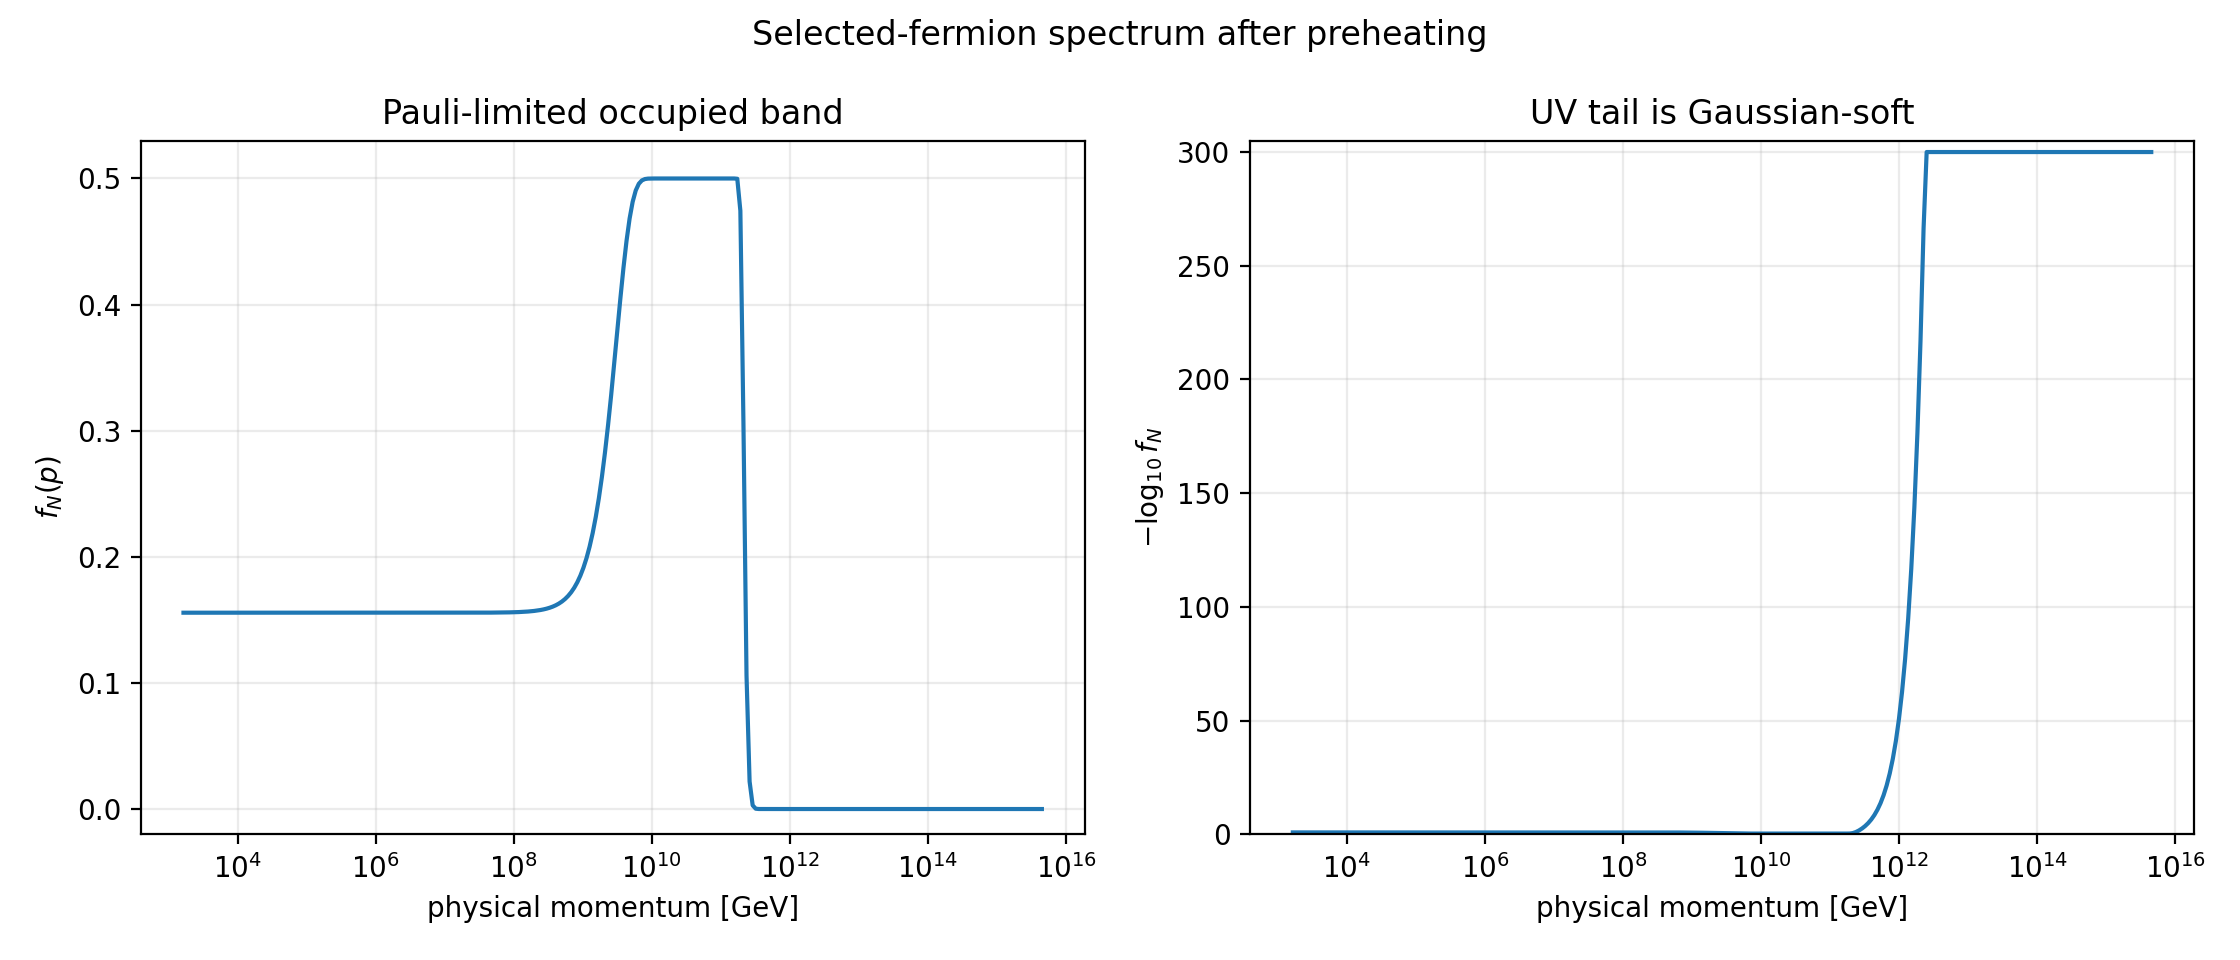
\includegraphics[width=0.98\textwidth,height=\textheight]{fermionic_preheating_spectrum_v1_2.png}
\caption{Selected-fermion occupation and its UV tail. The stochastic
update can transiently saturate the Pauli bound even though the final
energy fraction remains tiny.}
\end{figure}

\begin{figure}
\centering
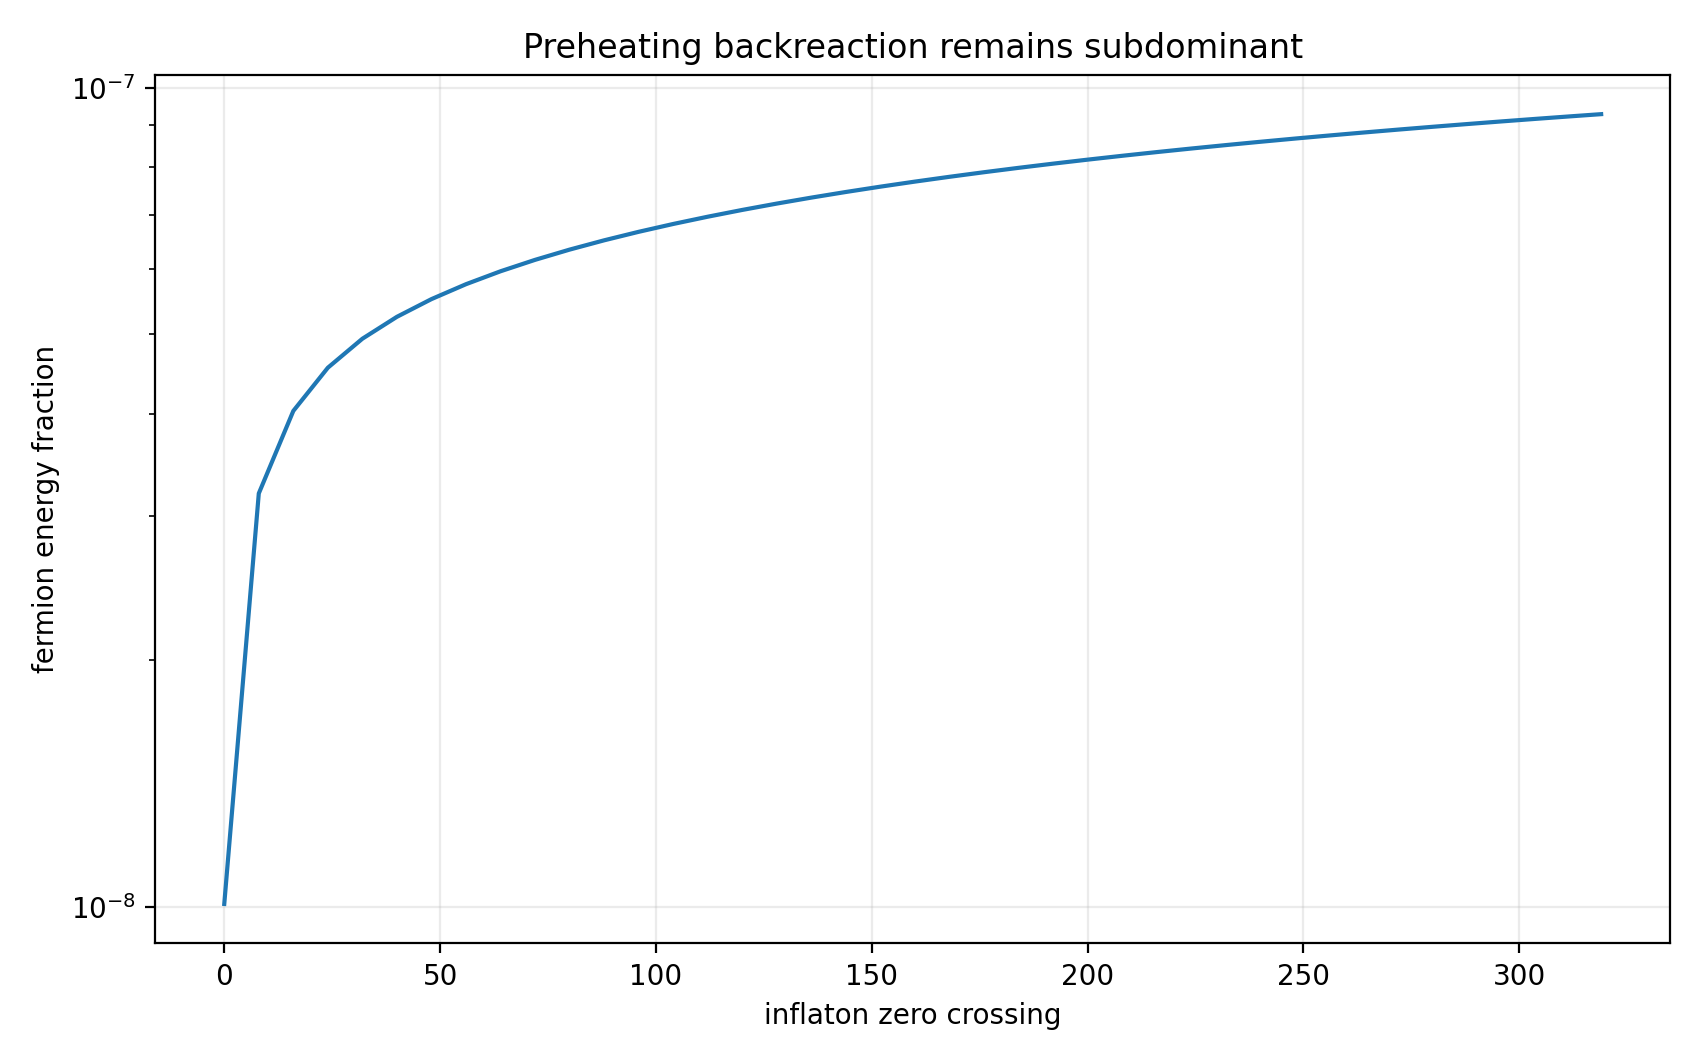
\includegraphics[width=0.82\textwidth,height=\textheight]{fermionic_preheating_backreaction_v1_2.png}
\caption{The preheating component remains below \(10^{-7}\) of the total
energy.}
\end{figure}

\section{5. Nonlinear radial momentum-lattice
cascade}\label{nonlinear-radial-momentum-lattice-cascade}

\subsection{5.1 Resolved chain}\label{resolved-chain}

The perturbative and plasma stages are

\[
\phi
\xrightarrow{\Gamma_\phi}
N_0\bar N_0,
\]

\[
N_0
\xrightarrow{\Gamma_N}
R_0+\nu_0,
\]

\[
R_0
\xrightarrow{\Gamma_R}
H_0H_0
\quad\text{or}\quad
H_5H_5,
\]

followed by the sector-local processes represented schematically by

\[
H_k+q_k\leftrightarrow D_k,
\qquad
D_k,q_k,g_k\leftrightarrow\text{plasma}_k.
\]

The benchmark rates are

\[
\Gamma_\phi=100\ {\rm GeV},
\quad
\Gamma_Q=1\ {\rm GeV},
\quad
\Gamma_N=0.10\ {\rm GeV},
\]

\[
\Gamma_R=1.4135\times10^{-2}\ {\rm GeV},
\quad
\Gamma_{\rm th}=0.25\ {\rm GeV}.
\]

The momentum lattice evolves the radial distributions in an expanding
FRW background. For an unstable particle of mass \(m\) and energy
\(E(p)\), the decay fraction over \(dt\) is

\[
1-
\exp\left[-\Gamma\frac{m}{E(p)}dt\right].
\]

Each two-body decay is deposited using the exact rest-frame momentum

\[
p_*
=
\frac{
\sqrt{[m_P^2-(m_1+m_2)^2][m_P^2-(m_1-m_2)^2]}
}{2m_P},
\]

boosted over an isotropic angular quadrature into daughter momentum
bins.

\subsection{5.2 Quantum-BGK plasma
closure}\label{quantum-bgk-plasma-closure}

The unresolved sector-local scattering network is represented by

\[
\left(\partial_t-Hp\partial_p\right)f_i
=
-\Gamma_{\rm th}
\left[f_i-f_i^{\rm eq}(T_k)\right],
\]

with Bose-Einstein or Fermi-Dirac targets as appropriate. The
temperature is solved from the instantaneous sector energy density. A
spectator bath carries degrees of freedom not explicitly resolved on the
four tracked distributions \(H,D,q,g\).

After each collision step, the spectator energy is corrected by the
numerical quadrature residual, making the closure energy conserving to
machine precision. This is a controlled kinetic surrogate, not a
derivation of the QCD collision kernel.

Quantum multi-species BGK models can be built to share the conservation
laws and \(H\)-theorem of the corresponding quantum Boltzmann system.
The present implementation uses that conservation logic while retaining
the actual expanding momentum lattice and decay kernels.

\subsection{5.3 Energy flow}\label{energy-flow}

\begin{figure}
\centering
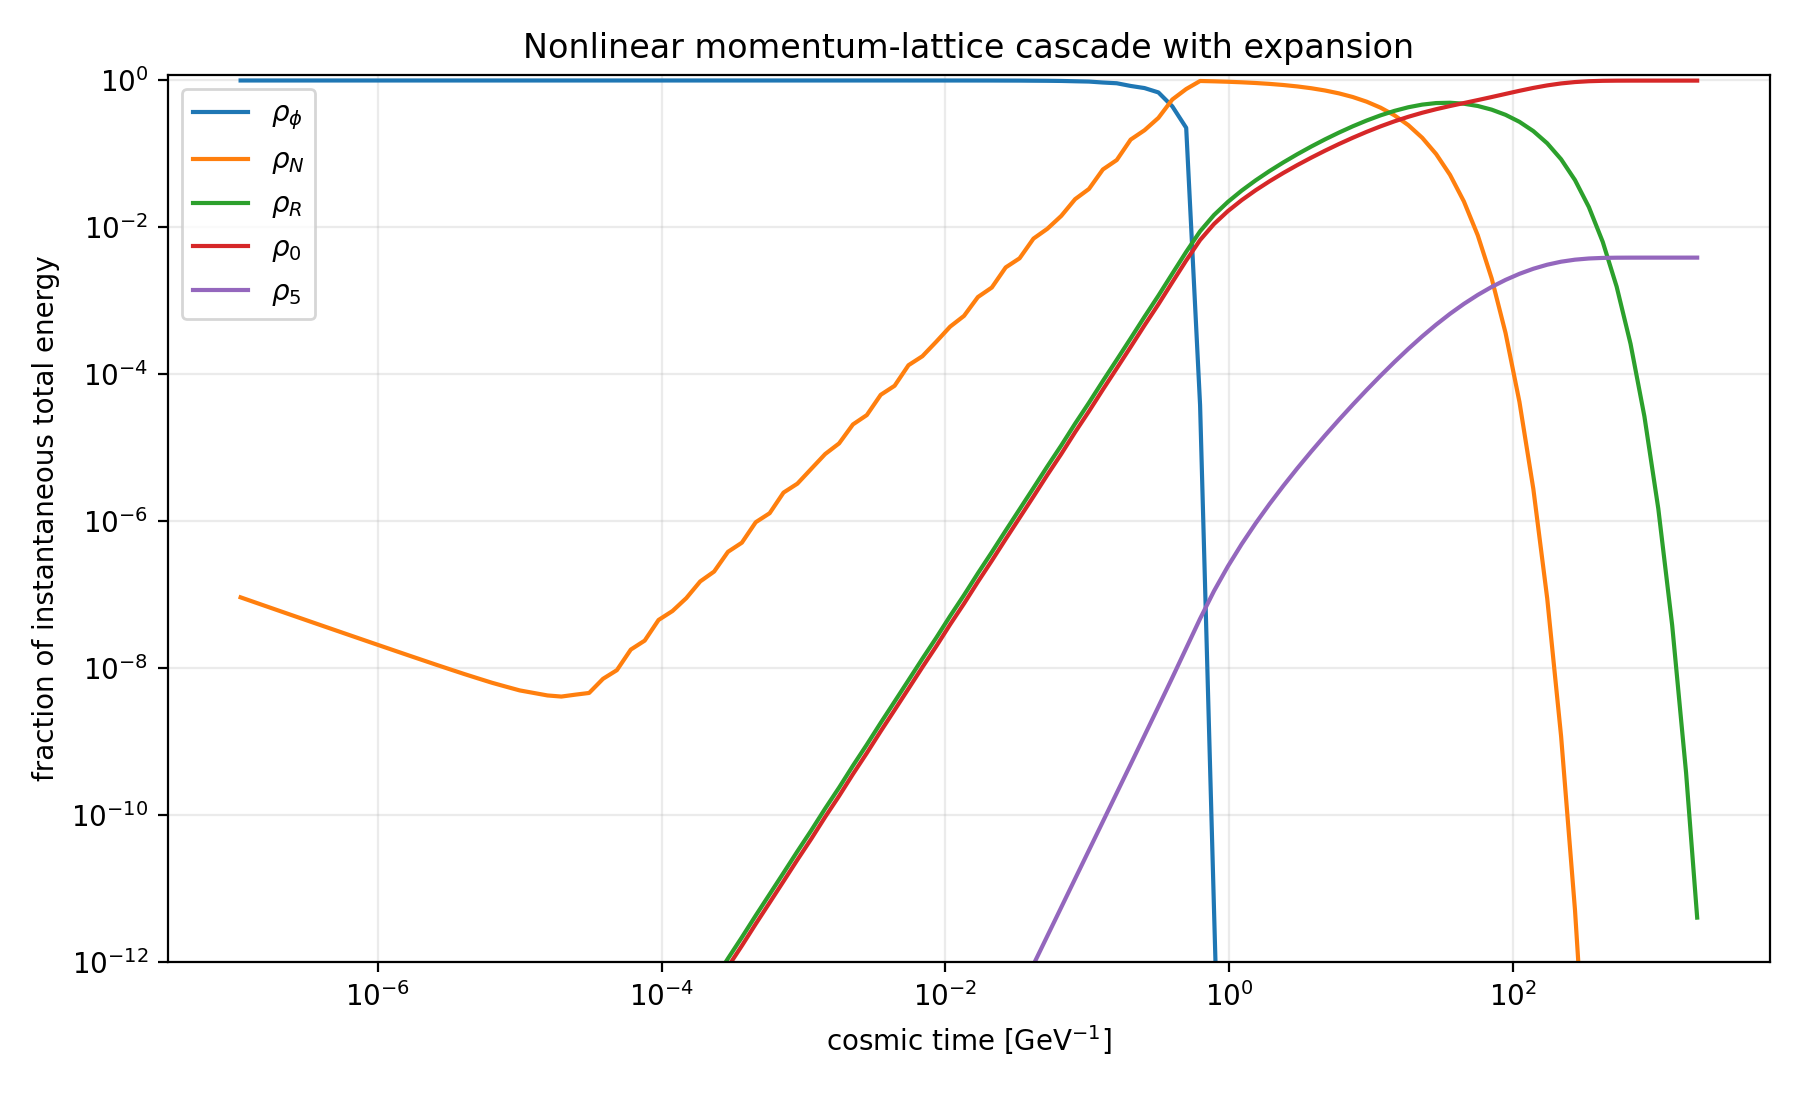
\includegraphics[width=0.9\textwidth,height=\textheight]{nonlinear_cascade_energy_flow_v1_2.png}
\caption{Fractions of the instantaneous total energy carried by each
stage of the cascade.}
\end{figure}

The evolution displays the intended sequence:

\begin{enumerate}
\def\labelenumi{\arabic{enumi}.}
\tightlist
\item
  inflaton domination;
\item
  transfer into \(N_0\);
\item
  delayed population of \(R_0\) and sector-0 radiation from \(\nu_0\);
\item
  decay of \(R_0\) into sectors 0 and 5;
\item
  thermalisation into the two replica plasmas.
\end{enumerate}

The selector charge has decayed to zero by the final state. The final
\(N_0\) and \(R_0\) energy densities are negligible.

\section{6. Cascade-corrected replica
branch}\label{cascade-corrected-replica-branch}

\subsection{\texorpdfstring{6.1 Why \(B_5=1/257\)
fails}{6.1 Why B\_5=1/257 fails}}\label{why-b_51257-fails}

For

\[
m_N=3\times10^9\ {\rm GeV},
\qquad
m_R=10^9\ {\rm GeV},
\]

the fraction of the parent energy carried by \(R\) in its rest frame is

\[
\boxed{
f_R
=
\frac{m_N^2+m_R^2}{2m_N^2}
=
\frac59.
}
\]

The massless \(\nu_0\) carries the remaining \(4/9\) into sector 0. It
is injected on the timescale \(\Gamma_N^{-1}\), while the \(R\) energy
is released later on the timescale \(\Gamma_R^{-1}\). The two
contributions therefore experience different redshift histories.

If the entire parent energy had been released by \(R\) at one time, the
old relation

\[
B_5=\frac1{257}
\]

would give \(E_5/E_0=1/256\). Once the \(\nu_0\) daughter is included,
this branch gives dynamically

\[
\frac{T_5}{T_0}=0.231634.
\]

Correcting only for the instantaneous rest-frame fraction would suggest

\[
B_5^{\rm inst}
=
\frac{1}{257f_R}
=0.00700389,
\]

but the full evolution then gives

\[
\frac{T_5}{T_0}=0.268455.
\]

It overshoots because the early \(\nu_0\) radiation has redshifted more
strongly by the time the \(R\) decay products dominate.

\subsection{6.2 Exact branch reconstruction from the lattice
response}\label{exact-branch-reconstruction-from-the-lattice-response}

Because the two replica sectors have identical post-injection dynamics,
the final sector energies are linear in the \(R\) branch. Let

\[
E_R^{(1)}
\]

be the final redshifted energy that would arise if all \(R\) decays fed
one sector, and let

\[
E_\nu
\]

be the final redshifted sector-0 energy from the earlier \(\nu_0\)
injection. The simulation gives

\[
\boxed{
\mathcal R_\nu
\equiv
\frac{E_\nu}{E_R^{(1)}}
=0.35551328.
}
\]

For branch \(B_5\),

\[
E_5=B_5E_R^{(1)},
\]

\[
E_0=E_\nu+(1-B_5)E_R^{(1)}.
\]

Imposing

\[
\frac{E_5}{E_0}=\frac1{256}
\]

gives

\[
\boxed{
B_5^*
=
\frac{1+\mathcal R_\nu}{257}
=0.00527437074.
}
\]

The value used in the final run is

\[
B_5=0.00527437084,
\]

whose independently reconstructed value differs by only

\[
1.97\times10^{-8}
\]

relatively. The corresponding reheaton mixing is

\[
\boxed{
\tan\theta
=
\sqrt{\frac{B_5}{1-B_5}}
=0.0728196.
}
\]

The final result is

\[
\boxed{
\frac{E_5}{E_0}=0.00390625008,
\qquad
\frac{T_5}{T_0}=0.250000001.
}
\]

\begin{figure}
\centering
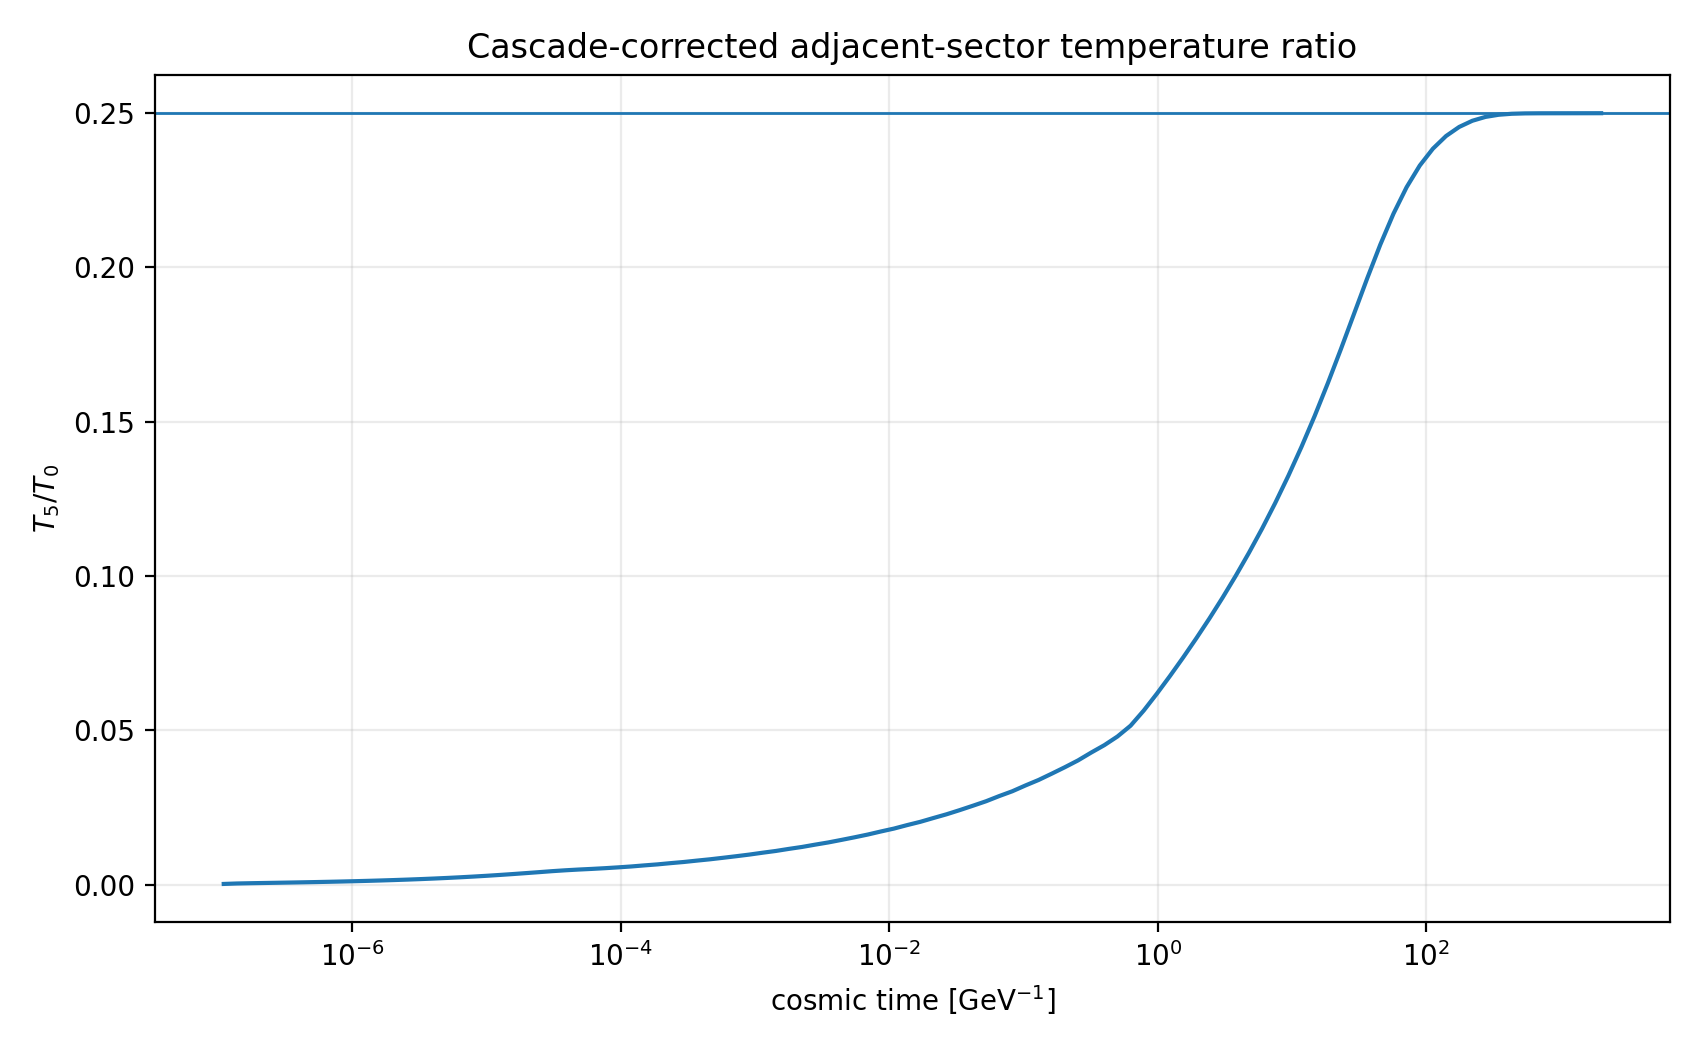
\includegraphics[width=0.84\textwidth,height=\textheight]{cascade_temperature_ratio_v1_2.png}
\caption{The full cascade approaches the target adjacent-sector
temperature ratio after the redshift-corrected branch is used.}
\end{figure}

This is a genuine model correction: the previously attractive exact
choice \(\tan\theta=1/16\) must be replaced once the full decay chain is
resolved.

\clearpage

\section{7. Final plasma state and numerical
controls}\label{final-plasma-state-and-numerical-controls}

\subsection{7.1 Energy partition}\label{energy-partition}

The final visible-sector energy fractions are

\begin{longtable}[]{@{}lr@{}}
\toprule\noalign{}
Component & Fraction of sector-0 energy \\
\midrule\noalign{}
\endhead
\bottomrule\noalign{}
\endlastfoot
\(H_0\) & 0.0374872 \\
\(D_0\) & 0.0983633 \\
\(q_0\) & 0.0984038 \\
\(g_0\) & 0.1499487 \\
unresolved spectator bath & 0.6157970 \\
\end{longtable}

The adjacent sector has the same partition to within the expected
finite-grid effects.

\begin{figure}
\centering
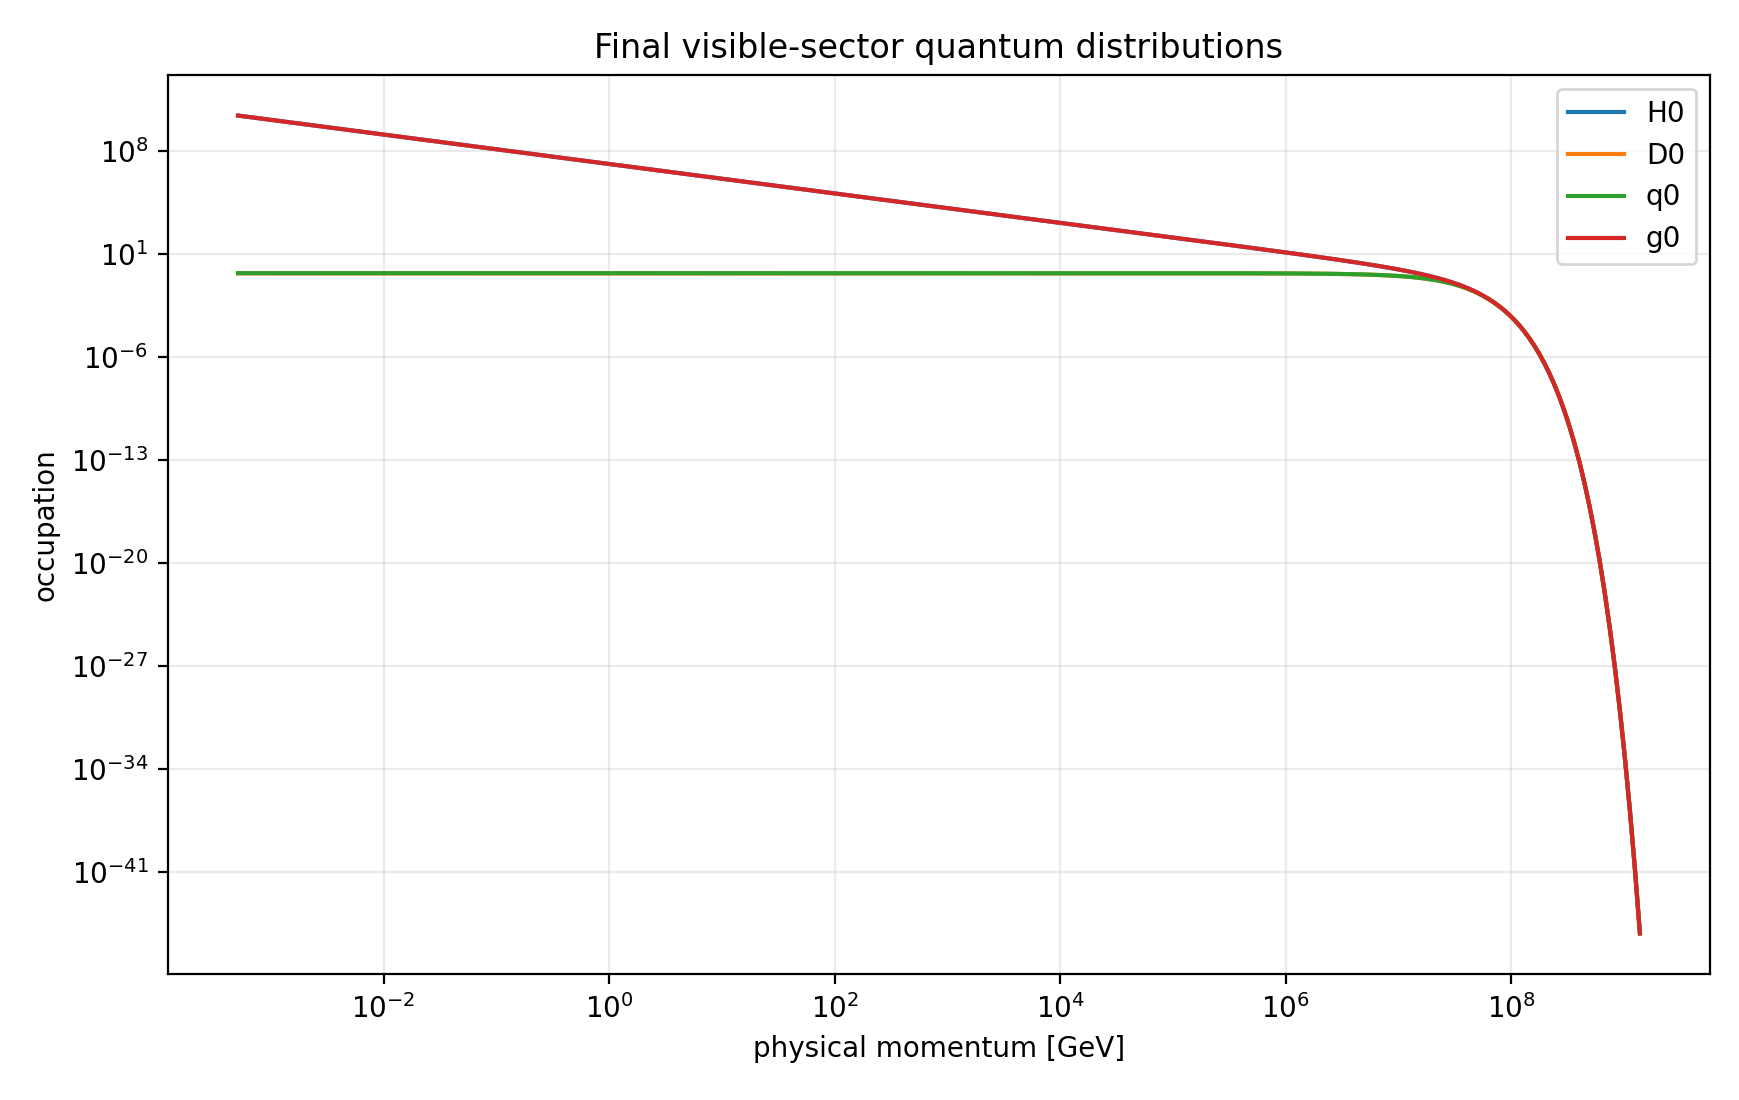
\includegraphics[width=0.88\textwidth,height=\textheight]{cascade_final_spectra_v1_2.png}
\caption{Final visible-sector occupation functions. The resolved
distributions have exponential thermal tails.}
\end{figure}

\clearpage

\begin{figure}
\centering
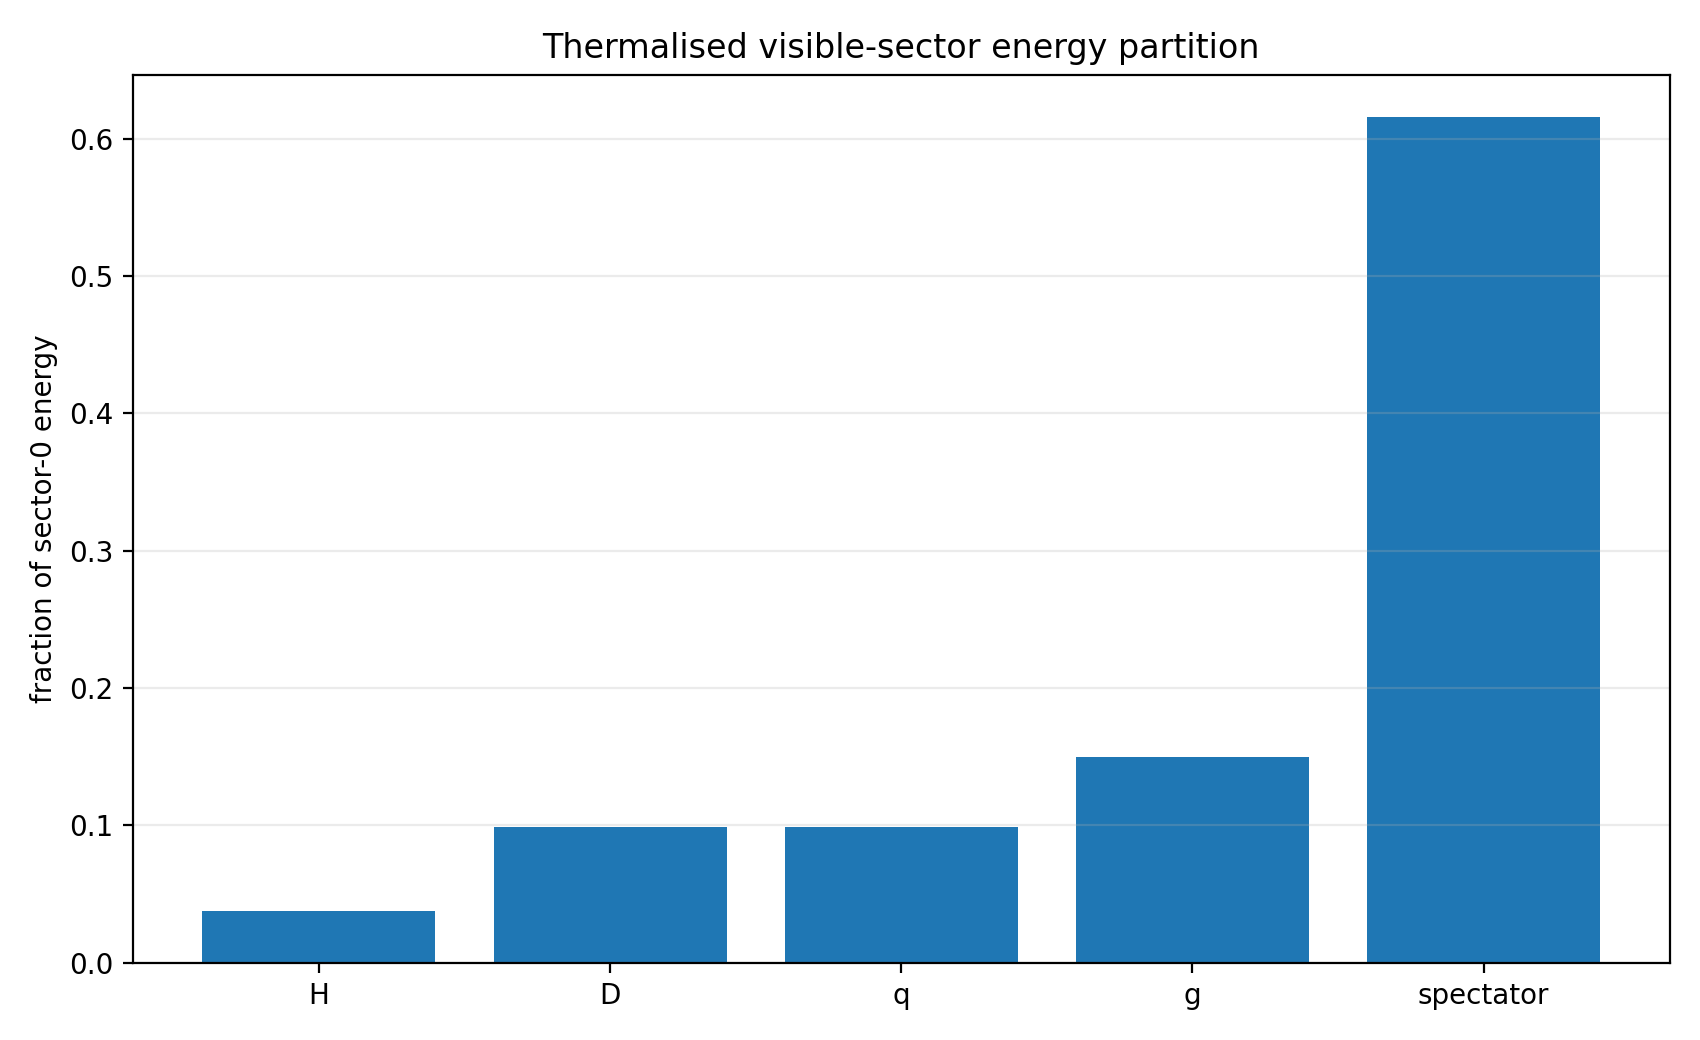
\includegraphics[width=0.84\textwidth,height=\textheight]{cascade_species_partition_v1_2.png}
\caption{Energy carried by the explicitly resolved species and the
unresolved relativistic spectator bath.}
\end{figure}

The fitted exponential tails satisfy

\[
R_H^2=0.999999976,
\qquad
R_g^2=0.99999999999998.
\]

\subsection{7.2 Conservation and positivity
diagnostics}\label{conservation-and-positivity-diagnostics}

The key numerical controls are:

\begin{longtable}[]{@{}lr@{}}
\toprule\noalign{}
Test & Result \\
\midrule\noalign{}
\endhead
\bottomrule\noalign{}
\endlastfoot
maximum Pauli occupation during preheating & 0.999929 \\
maximum two-body kinematic energy residual & \(5.59\times10^{-16}\) \\
maximum collision-step energy residual & \(1.73\times10^{-16}\) \\
hidden-parent production bound & \(\log_{10}P<-8562.6\) \\
Gaussian UV-tail fit & \(R^2=0.999992\) \\
final \(T_5/T_0\) & 0.250000001 \\
\end{longtable}

Attempted perturbative inflaton decays into already occupied fermion
bins are Pauli-throttled: rejected occupation is not destroyed but
remains in the inflaton energy density until expansion opens phase
space. The raw accumulated attempted rejection is therefore not itself a
physical relic abundance.

\section{8. Relation to a full Kadanoff-Baym
calculation}\label{relation-to-a-full-kadanoff-baym-calculation}

The radial momentum-lattice calculation evolves nonlinear occupation
functions, expansion, backreaction, exact two-body decays, Pauli
blocking, and an energy-conserving relaxation closure. It is materially
stronger than a homogeneous branching-fraction calculation.

It is nevertheless not the same object as a full 2PI/Kadanoff-Baym
evolution. A complete calculation would evolve unequal-time statistical
and spectral propagators,

\[
F_i(t,t';p),
\qquad
\rho_i(t,t';p),
\]

with nonlocal self-energies and memory integrals for the scalar,
fermion, and gauge sectors. Such equations conserve energy and global
charges when derived from a controlled 2PI truncation, but their full
\(3+1\)-dimensional numerical solution is an HPC-scale problem.

The next simulation layer should replace

\[
C_i^{\rm BGK}
\]

by either:

\begin{enumerate}
\def\labelenumi{\arabic{enumi}.}
\tightlist
\item
  explicit \(1\leftrightarrow2\) and \(2\leftrightarrow2\) collision
  integrals including thermal masses, LPM effects, and colour factors;
  or
\item
  a symmetry-preserving two-loop or three-loop 2PI truncation for the
  \(H,D,q,g\) system.
\end{enumerate}

\section{9. Initial-state
renormalisation}\label{initial-state-renormalisation}

The preheating benchmark produces a Gaussian-soft high-momentum tail. It
therefore does not show the logarithmic energy divergence associated
with an abrupt \(k^{-4}\) quench tail.

This does not eliminate initial-state renormalisation as a general
issue. In Schwinger-Keldysh perturbation theory, ultraviolet structure
specific to a non-vacuum initial state can require counterterms
localised on the initial hypersurface. Such terms renormalise the state
preparation; they do not automatically become permanent bulk vacuum
spurions.

The present benchmark passes the practical UV-tail test. A future
lattice preheating run should still extract the asymptotic tail at
increasing cutoff and verify convergence of:

\[
\rho,
\qquad
P,
\qquad
\langle\bar NN\rangle,
\qquad
\text{and the transient harmonic source}.
\]

\section{10. Status of the requested
targets}\label{status-of-the-requested-targets}

\begin{longtable}[]{@{}
  >{\raggedright\arraybackslash}p{(\columnwidth - 4\tabcolsep) * \real{0.3000}}
  >{\raggedleft\arraybackslash}p{(\columnwidth - 4\tabcolsep) * \real{0.4000}}
  >{\raggedright\arraybackslash}p{(\columnwidth - 4\tabcolsep) * \real{0.3000}}@{}}
\toprule\noalign{}
\begin{minipage}[b]{\linewidth}\raggedright
Target
\end{minipage} & \begin{minipage}[b]{\linewidth}\raggedleft
Verdict
\end{minipage} & \begin{minipage}[b]{\linewidth}\raggedright
Meaning
\end{minipage} \\
\midrule\noalign{}
\endhead
\bottomrule\noalign{}
\endlastfoot
identify the first mixed graph & \textbf{PASS} & three-loop 1PI,
two-particle reducible \\
calculate \(\mathcal I_3\) & \textbf{PASS in scalar proxy} & exact
factorised zero-momentum \(\overline{\rm MS}\) function \\
validate matching analytically & \textbf{PASS} & symbolic residual zero;
70-digit derivative check \\
calculate \(\gamma_{pq}^{\rm transient}\) & \textbf{PARTIAL} & exact
all-orders spurion-power selection and explicit one-loop scalar block;
finite gauge/Yukawa tensors open \\
show transient correction remains small & \textbf{PASS} &
\(|\Delta V^{(3)}|/V_{\rm thermal}=1.55\times10^{-12}\) \\
nonlinear fermion preheating & \textbf{PASS at radial kinetic level} &
Pauli blocking, expansion, and backreaction included \\
suppress unselected parents & \textbf{PASS} & exponent
\(>1.97\times10^4\) \\
nonlinear decay cascade & \textbf{PASS at radial kinetic level} & exact
two-body kernels and time dilation included \\
reproduce \(T_5/T_0=1/4\) & \textbf{PASS after branch correction} &
\(B_5=0.00527437\) \\
old \(\tan\theta=1/16\) & \textbf{FAIL} & omitted \(\nu_0\) energy and
differential redshift \\
full non-Abelian \(3+1\)D KB plasma & \textbf{OPEN} & requires
unequal-time 2PI/HPC implementation \\
fully RG-improved physical coefficient & \textbf{OPEN} & must combine
hard matching with complete operator running \\
\end{longtable}

\section{11. Scientific interpretation}\label{scientific-interpretation}

The calculation strengthens the central state-selection proposal in
three ways.

First, the first mixed selector-threshold vacuum correction is no longer
an order-of-magnitude guess:

\[
\mathcal I_3\sim1
\quad\longrightarrow\quad
\mathcal I_3(M)=6.57973508149.
\]

Despite the coefficient being larger than unity, the correction remains
twelve orders of magnitude below the intended thermal force because the
loop, portal, hierarchy, and \(\epsilon\) suppressions are severe.

Second, the renormalisation structure is now stated correctly. Exact
\(Z_6\) protects the vacuum charge structure, while approximate
continuous shift symmetry grades cross-harmonic mixing by explicit
powers of \(\epsilon\). This is sufficient for the benchmark, but it
does not excuse the calculation of the remaining finite operator
tensors.

Third, the full decay chronology matters. A branching fraction that is
exact at the \(R\) decay vertex is not automatically exact for the final
temperatures when an earlier daughter deposits energy asymmetrically.
The corrected branch is an output of the dynamical cascade, not a
cosmetic retuning.

The resulting picture is:

\[
\boxed{
\begin{aligned}
\text{vacuum action symmetry}
&\Rightarrow
\text{protected }p=6\text{ vacuum harmonic},\\
\text{selector/state asymmetry}
&\Rightarrow
\text{temporary }p=1\text{ focusing force},\\
\text{three-loop mixed matching}
&\Rightarrow
\text{tiny transient radiative correction},\\
\text{fermionic cascade}
&\Rightarrow
\text{controlled asymmetric population},\\
\text{full redshift history}
&\Rightarrow
\text{corrected }T_5/T_0=1/4.
\end{aligned}
}
\]

\section{12. Next decisive calculation}\label{next-decisive-calculation}

The next target should combine two previously separate gaps:

\[
\boxed{
\text{RG-improved transient matching}
+
\text{non-Abelian nonequilibrium transport}.
}
\]

Concretely:

\begin{enumerate}
\def\labelenumi{\arabic{enumi}.}
\tightlist
\item
  construct the complete local operator basis
  \(e^{ipx}\mathcal Q_{-p}\), \(e^{ipx}\mathcal Q_{-p}H^\dagger H\),
  \(e^{ipx}\mathcal Q_{-p}\bar DD\), and \(e^{ipx}\mathcal Q_{-p}G^2\),
  including evanescent and equation-of-motion operators as required;
\item
  calculate the one-loop and relevant two-loop \(\Gamma_{AB}^{(r,s)}\)
  tensors;
\item
  run the hard coefficient from \(m_R\) through \(M\) and the
  electroweak scale, verifying matching-scale cancellation;
\item
  replace the BGK closure with explicit thermal collision kernels or a
  2PI truncation;
\item
  scan \(\Gamma_N/\Gamma_R\), thermal masses, \(M_D/T\), and the
  selector decay profile to determine whether the corrected \(B_5\) is
  stable or shifts appreciably;
\item
  feed the resulting temperature and perturbation transfer functions
  back into the cosmological vacuum-selection calculation.
\end{enumerate}

\section{References}\label{references}

\begin{enumerate}
\def\labelenumi{\arabic{enumi}.}
\tightlist
\item
  S. P. Martin, \emph{Two-loop effective potential for a general
  renormalizable theory and softly broken supersymmetry}, Phys. Rev.~D
  65, 116003 (2002),
  \href{https://arxiv.org/abs/hep-ph/0111209}{arXiv:hep-ph/0111209}.
\item
  S. P. Martin and D. G. Robertson, \emph{Evaluation of the general
  3-loop vacuum Feynman integral}, Phys. Rev.~D 95, 016008 (2017),
  \href{https://arxiv.org/abs/1610.07720}{arXiv:1610.07720}.
\item
  P. B. Greene and L. Kofman, \emph{Preheating of Fermions}, Phys. Lett.
  B 448, 6 (1999),
  \href{https://arxiv.org/abs/hep-ph/9807339}{arXiv:hep-ph/9807339}.
\item
  P. B. Greene and L. Kofman, \emph{On the Theory of Fermionic
  Preheating}, Phys. Rev.~D 62, 123516 (2000),
  \href{https://arxiv.org/abs/hep-ph/0003018}{arXiv:hep-ph/0003018}.
\item
  J. Berges, \emph{Introduction to Nonequilibrium Quantum Field Theory},
  AIP Conf. Proc. 739, 3 (2004),
  \href{https://arxiv.org/abs/hep-ph/0409233}{arXiv:hep-ph/0409233}.
\item
  M. Lindner and M. M. Mueller, \emph{Comparison of Boltzmann Kinetics
  with Quantum Dynamics for a Chiral Yukawa Model Far From Equilibrium},
  Phys. Rev.~D 77, 025027 (2008),
  \href{https://arxiv.org/abs/0710.2917}{arXiv:0710.2917}.
\item
  H. Collins and R. Holman, \emph{Renormalization of initial conditions
  and the trans-Planckian problem of inflation}, Phys. Rev.~D 71, 085009
  (2005),
  \href{https://arxiv.org/abs/hep-th/0501158}{arXiv:hep-th/0501158}.
\item
  G.-C. Bae, C. Klingenberg, M. Pirner and S.-B. Yun, \emph{BGK model of
  the multi-species Uehling-Uhlenbeck equation}, Kinetic Relat. Models
  15, 25 (2022),
  \href{https://arxiv.org/abs/1912.01677}{arXiv:1912.01677}.
\end{enumerate}

\end{document}
